\chapter{Tracking}
\label{cap:tracking}
\thispagestyle{empty}

\begin{quotation}
{\footnotesize
\noindent\emph{Marty: Ma allora dove diavolo sono? \\
Doc: La domanda giusta è: 'Quando diavolo sono?'}
\begin{flushright}
Ritorno al Futuro, parte I
\end{flushright}
}
\end{quotation}
\vspace{0.5cm}

\section{Introduzione}

Una volta riconosciute le possibili feature, è necessario seguirle nelle immagini successive della telecamera.
Per farlo, ci siamo basati su un algoritmo presente in letteratura, chiamato Consensus-based Matching and Tracking, CMT~\cite{Nebehay2014WACV}.
L'algoritmo considerato è un algoritmo di tracking a lungo termine. Gli algoritmi di tracking a lungo termine permettono di inseguire oggetti che entrano e escono dal campo visivo della telecamera, e cercano di discriminare anche tra oggetti simili.

Il tracker implementato è in grado non solo di riconoscere gli oggetti nell'immagine, ma è in grado, in parte, di capire se gli oggetti riconosciuti dall'algoritmo descritto nel \autoref{cap:riconoscimento} sono già o meno nella lista ddegli oggetti da seguire.

In questo capitolo spiegheremo brevemente come funziona l'algoritmo CMT utilizzato e come è stato integrato con il riconoscimento di oggetti e con la costruzione della mappa.

\section{CMT}

L'idea base dell'algoritmo è che i keypoint siano un buon modo per scomporre in parti l'oggetto da seguire. Il primo passo consiste quindi nell'estrarre keypoint dal bounding box iniziale, calcolare i relativi descrittori delle feature e salvare tutto in un database. Questa idea è resa possibile dal recente sviluppo di algoritmi veloci ed efficienti per l'estrazione di feature quali~\cite{rosten_2006_machine} e~\cite{6126542}.

Successivamente, per ogni frame, i keypoint presenti nell'iterazione precedente vengono inseguiti tramite il calcolo del flusso ottico~\cite{Lucas:1981:IIR:1623264.1623280} di Lukas-Kanade, nella variante piramidale~\cite{Bouguet00pyramidalimplementation}. Inoltre vengono estratti keypoint e effettuato il matching con i keypoint presenti nel database. I keypoint di cui è stato effettuato con successo il matching vengono sostituiti a quelli seguiti tramite il flusso ottico, poiché si suppone che siano più stabili, non essendo parte di un processo iterativo di valutazione, soggetto ad errore integrale.

La seconda fase consiste in una procedura di votazione per determinare il centro di massa dell'oggetto.
In primo luogo vengono stimate la scala e la rotazione planare dell'oggetto, calcolando la variazione di scala e di rotazione tra tutte le coppie di keypoint e calcolandone la mediana. In seguito, ogni keypoint vota il centro di massa dell'oggetto utilizzando la sua posizione relativa al centro di massa nel primo frame, opportunamente scalato e ruotato grazie ai due valori precedentemente calcolati.

La terza fase dell'algoritmo consiste nell'eliminazione degli outlier tramite un meccanismo di consenso. I centri di massa votati da ciascun singolo keypoint vengono divisi in cluster in base alla distanza euclidea. Quindi, viene individuato il cluster con il maggior numero di voti. Se il cluster scelto ha un numero sufficiente di keypoint, allora l'oggetto viene considerato come visibile e viene calcolato il centro di massa dell'oggetto, eliminando tutti i voti che non appartengono al cluster.

Infine, il bounding box dell'oggetto viene calcolato applicando la rotazione e la scala calcolate precedentemente ai punti del bounding box iniziale. Questo procedimento è il punto più debole dell'algoritmo, perché il bounding box calcolato non tiene conto dell'omografia che può esserci tra il bounding box iniziale e quello attuale, causata, ad esempio, dalla distorsione prospettica a seguito della nuova posa della telecamera.

La nostra implementazione si discosta dall'implementazione originale, su cui è fortemente basata, solo per la possibilità di specificare un bounding box con una forma arbitraria.

\section{Integrazione con il riconoscimento degli oggetti}

L'algoritmo di tracking deve essere in grado di interagire con il riconoscimento a basso e alto livello degli oggetti. Per ottenere questo risultato abbiamo implementato alcune euristiche per gestire a basso livello e in maniera semplice i possibili conflitti tra l'algoritmo di tracking e il riconoscimento.

In primo luogo, per facilitare sia il tracking dell'oggetto, sia il riconoscimento ad alto livello, quando il tracker considera un nuovo oggetto da seguire inviato dal riconoscimento a basso livello, non utilizza il bounding box esatto riconosciuto, ma questo viene maggiorato, scalandolo, in modo da ottenere due importanti risultati:

\begin{enumerate}
 \item Riuscire a riconoscere in maniera efficiente i keypoint che si trovano sui bordi degli oggetti, che spesso sono i keypoint più significativi, soprattutto negli oggetti planari e uniformi, principali obbiettivi di questa tesi.
 \item Riuscire a compensare parzialmente il problema causato dal cambio di posa della telecamera, che potrebbe causare la fuoriuscita dell'oggetto, o parte di esso, dal bounding box, a causa della deformazione prospettica, non calcolata dall'algoritmo.
\end{enumerate}

Le track inviate al riconoscimento di alto livello comprendono due informazioni: il bounding box (maggiorato) e la regione di interesse rettangolare che lo contiene. Questo permette al riconoscimento di alto livello di analizzare solo le regioni di interesse rettangolari dell'immagine, rendendo il compito meno oneroso computazionalmente e di cancellare eventuali feature esterne all'oggetto, che non sono di interesse per il riconoscimento.

L'ultimo problema riguardante l'integrazione, il più problematico, è riuscire a discriminare quali oggetti riconosciuti sono già presenti nella lista delle track.

Questo problema può essere risolto a due livelli. Ad alto livello, è possibile capire che due oggetti tracciati nella mappa occupano lo stesso spazio, e quindi sono lo stesso oggetto. Questa è la soluzione ottimale, ma richiede un grande numero di informazioni e ha un costo computazionale elevato. 
Tuttavia è possibile affrontare a basso livello il problema, almeno parzialmente, escludendo in maniera semplice gli oggetti riconosciuti, con una euristica che abbiamo sviluppato. 
Questa si basa sul calcolo della posizione del centro di massa degli oggetti riconosciuti e delle track, rispetto ai loro bounding box.
Se un oggetto riconosciuto ha il suo centro di massa all'interno di un bounding box di una track attiva, o, viceversa, se una track attiva ha il suo centro di massa nel bounding box dell'oggetto riconosciuto, tale oggetto è considerato già seguito, e non viene aggiunto alla lista delle track.

\begin{figure}[ht]
  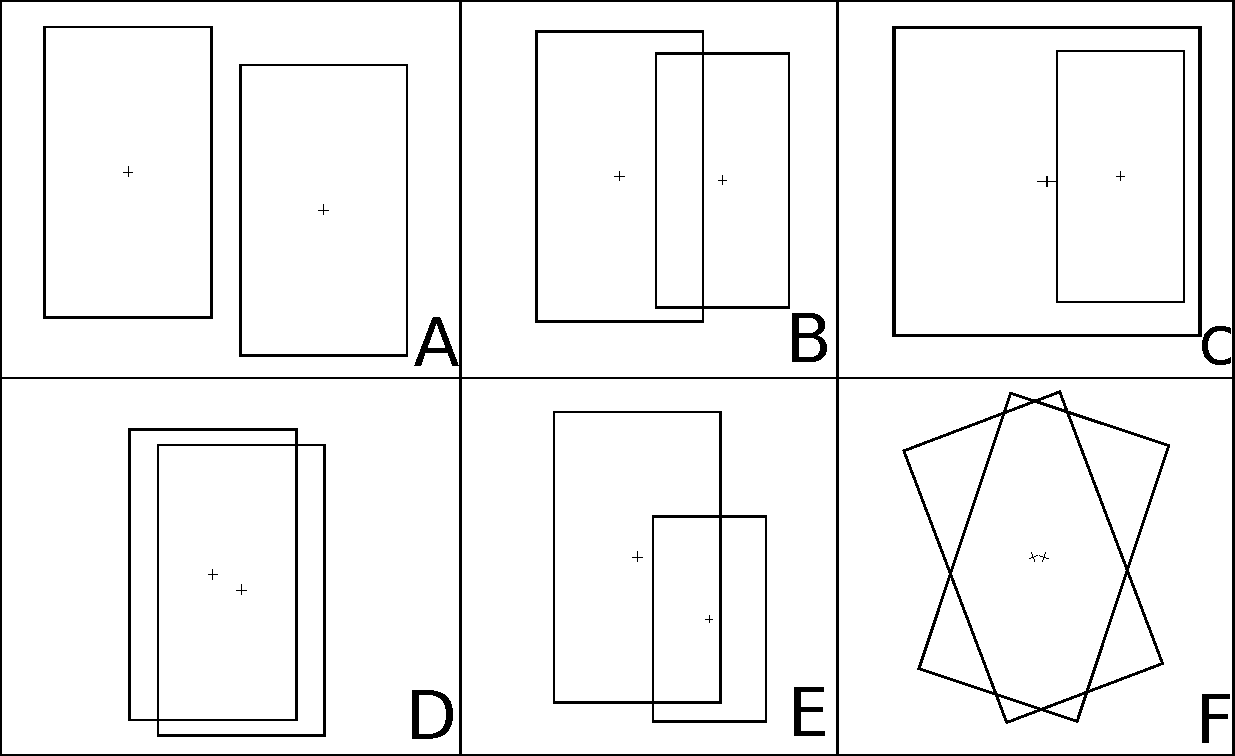
\includegraphics[width=\textwidth]{diagrammi/Euristica}
  \caption[Euristica del tracker]{I possibili posizionamenti delle due track: A. due oggetti differenti e distanti, B. due oggetti differenti abbastanza vicini, con parte del bounding box in comune, C. un oggetto contenente o con di fronte un altro oggetto, D. e F. lo stesso oggetto con due bounding box differenti, E. due oggetti differenti sovrapposti, lo stesso oggetto individuato male oppure un oggetto con una sua parte}
  \label{fig:euristica}
\end{figure}

Come si può vedere dalla \autoref{fig:euristica}, l'euristica copre abbastanza bene quasi tutti i casi, a parte quando si tratta di oggetti composti da più oggetti, o di oggetti che si trovano di fronte ad altri oggetti. Per questi casi sono necessari due ragionamenti ad alto livello differenti: riuscire a capire che un oggetto è semanticamente composto da alcune parti; riuscire a capire che i due oggetti non occupano lo stesso spazio. Per entrambi i ragionamenti non bastano le informazioni estratte dalla singola immagine.

\section{Integrazione con la mappa}
L'euristica descritta nel paragrafo precedente dimostra di comportarsi molto bene nelle situazioni reali, tuttavia subentrano alcuni problemi quando il tracking degli oggetti presenta dei mancati riconoscimenti. Questo causa spesso la sovrapposizione di più track dello stesso oggetto. Questo problema si può risolvere solamente integrando l'algoritmo di tracking con la mappa degli oggetti riconosciuti. Tramite la mappa è facile accorgersi che lo stesso oggetto è seguito più volte, poiché occupa la stessa posizione assoluta dell'oggetto seguito in precedenza.

Il tracking degli oggetti è un compito abbastanza oneroso computazionalmente. Se la posizione del robot è nota, anche in maniera imprecisa, non è necessario mantenere attivo l'algoritmo di tracking per tutti gli oggetti. Inoltre, l'algoritmo usato è soggetto a falsi positivi; potendo filtrare le track che non possono essere attive, perché non si trovano nell'area vista dal robot in un determinato istante, il tasso di falsi positivi cala drasticamente.

Infine, grazie alla stima della posizione, si può calcolare l'omografia che tiene conto della deformazione prospettica del bounding box dell'oggetto rispetto al nuovo punto di vista. Così facendo si può facilitare il riconoscimento ad alto livello.
